\documentclass{article}
\usepackage{graphicx}
\usepackage{float}
\usepackage{amsmath}
\usepackage{amssymb}
\usepackage{hyperref}
\usepackage{xcolor}
\usepackage{todonotes}
\usepackage{subfig}
\usepackage{caption}
\usepackage[ruled]{algorithm2e}
\title{Face Image Fitting\footnote{This is the first time we try to write the course project report in English. Your understanding is much appreciated.}}
\author{Kangcheng Hou\footnote{kangchenghou@gmail.com} \and Shuqi Wang\footnote{wangshuqi.cn@gmail.com} \and Tianhao Wei \footnote{phi.wth@gmail.com}}
\date{\today}
 

\newcommand{\pic}[2] {
    \begin{figure}[H]
    \centering
    \includegraphics[width=.6\textwidth]{./img/#1}
    \caption{#2}
    \end{figure}
}

\DeclareMathOperator*{\argmax}{arg\,max}
\DeclareMathOperator*{\argmin}{arg\,min}

\begin{document}

\maketitle
\tableofcontents

\section{Introduction}
A large proportion of images people uploaded is facial images. Motivated by this, in this course project, we want to develop a software that ease the process of editing facial image. The core part of our course project is face fitting, i.e. given a image, find the corresponding 3D model of the image. We also build two applications based upon the face fitting module.

The first one is to substitute the mouth in one image to another. The second one is to provide accessible way to edit face.
\begin{figure}
    \centering
    \subfloat[]{\includegraphics[width=0.4\textwidth]{./img/app11}}
    \hfill
    \subfloat[]{\includegraphics[width=0.4\textwidth]{./img/app12}}
    \caption{One application of face fitting is to transfer the smile from face (a) to face (b)}
\end{figure}
\begin{figure}
    \centering
    \subfloat[]{\includegraphics[width=0.4\textwidth]{./img/app21}}
    \hfill
    \subfloat[]{\includegraphics[width=0.4\textwidth]{./img/app22}}
    \caption{Another application of face fitting is to easily manipulate the face image without much artifact.}
\end{figure}

\subsection{Structure of the report}
In this report, we will first introduce the core part of this project, i.e. to reconstruct the 3D face model from a single image. Then we will introduce pipelines of two applications and their underlying techniques. Lastly, we will discuss further possible improvements of this project.
     

\section{Model fitting}
\subsection{Introduction}
Given a photo, we want to find a facial model fitted to the image. The typical method previously used is to first find the 2d feature points of the face and fit the 3d model to the image.

\begin{figure}[H]
\minipage{0.33\textwidth}
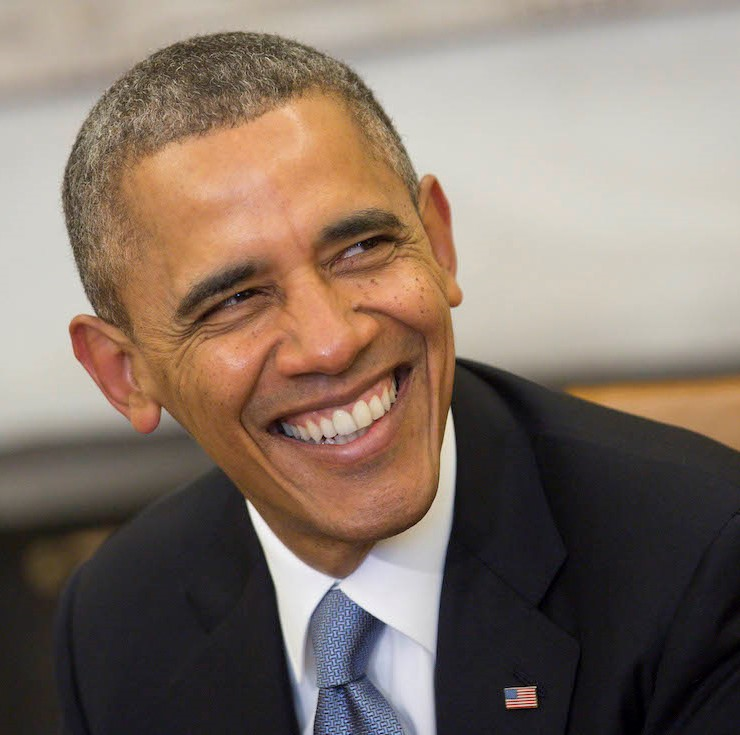
\includegraphics[width=\linewidth]{./img/img}
\endminipage\hfill
\minipage{0.33\textwidth}
\includegraphics[width=\linewidth]{./img/img_lm}
\endminipage\hfill
\minipage{0.33\textwidth}
\includegraphics[width=\linewidth]{./img/img_model}
\endminipage
\caption{The image, feature points and the fitted model}
\end{figure}
We first use state-of-the-art commercial software provided by face++\footnote{https://www.faceplusplus.com.cn/} to track the feature points $L^{(1), \cdots, (K)}$ which can be seen from the figure. Note that we include the points on the contour. As we will see later, feature points on the contour will be very helpful for fitting the model. Then we will fit a 3D model based on these points.

\subsection{Parametric Face Model}
Parametric face model use a low dimensional vector to represent different face model in the database. Previously methods use PCA or tensor decomposition to represent face model using low dimensional vectors. We use the Basel Face Model available online\footnote{https://faces.cs.unibas.ch/bfm/}. The basel face model provides us the mean face model $\overline{M}$, the identity principle components $\mathbf{V}_{\text{id}}$, the corresponding identity variations $\sigma^{\text{id}}$, the expression principle componets $\mathbf{V}^{\text{expr}}$, the corresponding expression variations $\sigma^{\text{expr}}$. The generating morphable model we use is 
$$M = \overline{M} + \mathbf{V}^{\text{id}} \times \mathbf{w}^{\text{id}} + \mathbf{V}^{\text{expr}} \times \mathbf{w}^{\text{expr}} \quad [\mathbf{w}^{\text{id}},\mathbf{w}^{\text{expr}}] \sim \mathcal{N}(0,\text{diag}([\Sigma^{\text{id}}, \Sigma^{\text{expr}}]))$$
Given the generating process of the 3D model, to fit the model to the 2D landmarks, we define the energy function to be optimized as follows.
$$E_{\text{fit}}(\textbf{w}) = \sum_i ||L_i - s\cdot(R \cdot M_{c(i)} + t)||_2^2 + \lambda \frac{1}{2}\mathbf{w}^\top \Sigma \mathbf{w}$$
\todo{add "for convenience, we will denote $\mathbf{w}$ as the concatenation of $\mathbf{w}^{\text{id}}$ and $\mathbf{w}^{\text{expr}}$}
where $s, R, t$ is camera parameters which we will introduce later, the parameter $\lambda$ balances the fitness to the data and the prior constraint and $c(i)$ find the corresponding index in the model w.r.t the ith landmark. 

\subsection{The General Procedure}
There is no closed form solution to the energy function mentioned above. We adopt the coordinate descent method to optimize this energy function. Coordinate descent works in similar way of Gibbs Sampling, i.e., iteratively fixing other variables except one and optimize the energy function w.r.t that variable. Our algorithm can be summerized as follows:

\begin{algorithm}[H]
\KwIn{facial landmarks $L^{(1), \dots, (K)}$ and the shape PCA model}
\KwOut{shape $M$ that best fits the landmarks and the corresponding camera parameters $s,R,t$}
Set $\mathbf{w} = 0$\;
\Repeat{$\mathbf{w}$ converges}{
    Set $\hat{M} = \bar{M} + \mathbf{V} \times \mathbf{w}$\;
    Find the camera parameters $s, R, t$ from $\hat{M}$ and $L^{(1), \dots, (K)}$ by using the least squares method\;
    Project all vertices of $\hat{M}$ onto the image plane: $\hat{M}' = \Pi_{R,s,t}(\hat{M})$\;
    Find the convex hull of $\hat{M}'$ as $H(\hat{M}')$\;
    For contour landmarks $L_i$, find correspondence using $H(\hat{M}')$\;
    Solve $\mathbf{w}$ using the energy function defined above.
}   
\caption{Fit the model to a single image}
\end{algorithm}

Knowing this general procedure, we now introduce what algorithm we use for seperate procedure.

\subsection{The Camera Model}
Before introducing the method of finding the camera parameter $s,R,t$. We first introduce the camera model we use. Like many previous work, we use the weak perspective camera model.\todo{Figure out this later} In weak perspective camera model, the transformation between 2D points and 3D points is specified by three parameters: scale $s$, rotation $R$, translation $s$. The transformation is specified as follows:
$$l = \Pi_{s,\mathbf{R},t}(m) = s \mathbf{R} m + t$$
This is based on the assumption that the object is far enough and no camera distortion is involved which is reasonable for modern camera setting and most applications.
\subsection{Finding the camera parameters}
Given the vertices on the 3D model $M_1, \dots, M_N$ and the corresponding landmarks $L_1, \dots, L_N$, we want to find the camera parameters $s, R, t$ that minimizes the fitting error.
$$ s, R, t = \argmin_{s,R,t} \sum_{i=1}^N|| L_i - \Pi_{s,R,t}(M_i)||_2^2$$
\todo{SVD decomposition} 

\subsection{Solve the $\mathbf{w}$}
Given the corrspondence, the camera parameters $s, R, t$, we can formulate the problem of solving $\mathbf{w}$ as a least square problem and solve it easily.


\section{Joint fitting of the model}
In some scenerios where we want to fit models for the same person that appeared in multiple images at the same time. We will need to fit the same identity weights $\mathbf{w}^{\text{id}}$ and fit the expression weights $\mathbf{w}^{\text{expr}}$ for different images. We adapt the previous algorithm as follows.

\section{Introduction of the applications}
Now we can fit a face model for a single image or fit multiple face models of the same person in multiple images, now we can do some interesting things. In the following sections, we will introduce three applications related to face model fitting and show the versatility of face fitting results.

\section{Face Image Editing}
Do some introduction of face image editing.
\subsection{Lapalacian Mesh Editing}

\subsection{Face IK}

\subsection{Results}



% \section{Mesh Deformation}
To enable easy facial animation, we tried out different methods of mesh deformation. We have tried the following methods:
\begin{itemize}
\item Face IK
\item Laplacian Mesh Editing
\item ARAP Mesh Deformation
\end{itemize}
The setting of our application is as follows, we specify some constraint pairs on the face mesh. Then we want to find a new mesh that satisfies the constraint while \textbf{looks similar} to the original mesh. Vertices on the original mesh is $\hat{\mathbf{x}}$ and the unknown vertices position of the deformed mesh is $\mathbf{x}$. And we can write the deformation field as $\hat{\mathbf{x}} - \mathbf{x} =: d$. We can think of the deformation process in two complementary way:
\begin{itemize}
\item Think about $d = \hat{\mathbf{x}} - \mathbf{x}$. Scattered data interpolation problem, where the constraint points specify constraints on the field $d$. Say $d_1 = u_1, \cdots, d_n = u_n$.
\item Think about the unknown vertices $\mathbf{x}$. The reconstructed mesh should satisfies the constraint while preserving some kind of details.
\end{itemize}

\subsection{Face IK}


\subsection{Biharmonic mesh deformation}


\subsection{ARAP deformation}




\bibliographystyle{apalike}
\bibliography{ref}

\end{document}